\chapter{Αξιολόγηση Συστήματος}
Στο κεφάλαιο αυτό γίνεται αξιολόγηση του μηχανισμού συστάσεων του συστήματος που υλοποιήσαμε 
για τις προσωποποιημένες προτάσεις άρθρων ειδήσεων σε μεμονωμένους χρήστες. \\

Εφόσον ο στόχος του συστήματος είναι η παραγωγή χρήσιμων ως προς τους χρήστες συστάσεων, 
πραγματοποιήσαμε ένα πείραμα για να ελέγξουμε την ακρίβεια της λειτουργίας αυτής. 
Το πείραμα βασίστηκε στην αξιολόγηση του συστήματος από 50 χρήστες.
Οι εθελοντές χρήστες εισήλθαν στο σύστημα, επέλεξαν προς ανάγνωση άρθρα της αρεσκείας τους 
και το σύστημα τα καταχώρησε στο αναγνωστικό τους ιστορικό. 
Στη συνέχεια, το σύστημα δημιούργησε σύνολα προτάσεων για καθέναν από αυτούς. 
Η ικανοποίηση κάθε χρήστη υπολογίσθηκε ως προς τα εξής τρία κριτήρια: 
\begin{itemize}
  \item Συσχετισμός των προτεινόμενων άρθρων με τα πραγματικά του ενδιαφέροντα ({\en {Preference}})
  \item Ποικιλία της λίστας συστάσεων ({\en {Diversity}})
  \item Kατάταξη των άρθρων της λίστας συστάσεων ({\en {Ordering}})
\end{itemize}

\newpage

Τα αποτελέσματα του πειράματος παρουσιάζονται στο παρακάτω ιστόγραμμα: \\

\begin{figure}[!ht] \centering
\centerline{
    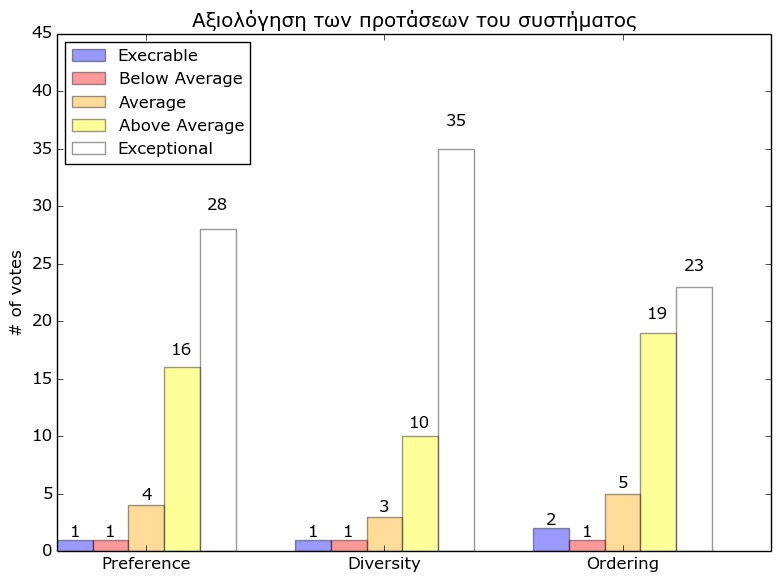
\includegraphics[scale=0.7]{static/figures/plots/plot1.png}}
    \caption{Αξιολόγηση των προτάσεων του συστήματος.}
    \label{}
\end{figure} 

Το συμπέρασμα που εξάγουμε από την πειραματική διαδικασία είναι ότι 
η πλειοψηφία των χρηστών επωφελείται από τις συστάσεις που παράγει το σύστημα, 
καθώς το μεγαλύτερο ποσοστό των χρηστών δηλώνει ικανοποιημένο ως προς τις απαιτήσεις 
για άρθρα σχετικά με τα ενδιαφέροντά του, ποικιλία στη λίστα συστάσεων 
και σωστή κατάταξη των άρθρων στην τελική λίστα. 
Συγκεκριμένα, ιδιαίτερα ικανοποιητικά είναι τα αποτελέσματα σχετικά με την ποικιλία της λίστας 
συστάσεων, όπου το σύστημα φαίνεται να εναρμονίζεται πλήρως με τα 
ενδιαφέροντα του χρήστη και να μην αφήνει καμία απ'τις ενδιαφέρουσες κατηγορίες 
άρθρων εκτός της τελικής σύστασης. \\

Άξιο καταγραφής αποτελεί και το πώς διαμορφώνονται οι συστάσεις προς έναν χρήστη 
κατά το χρόνο παραμονής του στο σύστημα, όπου δέχεται συστάσεις και συνεχίζει 
την ανάγνωση άρθρων. 
Κάθε λίστα συστάσεων περιέχει άρθρα από το πολύ τρεις διαφορετικές κατηγορίες, 
λαμβάνοντας υπόψη την τάση των χρηστών να προτιμούν συγκεκριμένες κατηγορίες άρθρων. \\

Στον Πίνακα 5.1 αποτυπώνονται οι πληροφορίες που αφορούν έναν τυχαίο χρήστη 
τη στιγμή που επιλέγει για πρώτη φορά να δεχθεί τις συστάσεις άρθρων του συστήματος. 
Στον πίνακα καταγράφονται το ιστορικό ανάγνωσης του χρήστη, 
δηλαδή ο αριθμός των άρθρων που έχουν αναγνωσθεί από κάθε κατηγορία έως τη δεδομένη στιγμή, 
η τιμή ομοιότητας του χρήστη με κάθε κατηγορία άρθρων, καθώς και ο αριθμός προτεινόμενων άρθρων 
από τις επιλεγμένες τρεις κατηγορίες με τη μεγαλύτερη ομοιότητα. \\

% ============================== 1 ===================================
\begin{table}[h]
\centering
\begin{center}
\begin{tabular}{|c|c|c|c|}
\hline
\cellcolor{blizzardblue}{\textit{\en {1st Recommendation}}}
& \multicolumn{1}{|p{3cm}|}{\centering \textbf{{\en {\# of articles }} \\ {\en {in user's}} \\ {\en {history}}}} 
& \multicolumn{1}{|p{3cm}|}{\centering \textbf{{\en {Similarity }} \\ {\en {with}} \\ {\en {Category}}}} 
& \multicolumn{1}{|p{3cm}|}{\centering \textbf{{\en {\# of }} \\ {\en {recommended articles}}}}\\
\hline
\multicolumn{1}{|p{3.8cm}|}{\centering \textbf{{\en {Category \#}1}}} & 4 & 0.2607 & 0 \\
\hline
\rowcolor{classicrose}
\multicolumn{1}{|p{3.8cm}|}{\centering \textbf{{\en {Category \#}2}}} & \textbf{6} & \textbf{0.3544} & \textbf{3} \\
\hline
\rowcolor{classicrose}
\multicolumn{1}{|p{3.8cm}|}{\centering \textbf{{\en {Category \#}3}}} & \textbf{7} & \textbf{0.3638} & \textbf{4} \\
\hline
\multicolumn{1}{|p{3.8cm}|}{\centering \textbf{{\en {Category \#}4}}} & 4 &  0.2469 & 0 \\
\hline
\multicolumn{1}{|p{3.8cm}|}{\centering \textbf{{\en {Category \#}5}}} & 4 & 0.3427 & 0 \\
\hline
\rowcolor{classicrose}
\multicolumn{1}{|p{3.8cm}|}{\centering \textbf{{\en {Category \#}6}}} & \textbf{4} & \textbf{0.3466} & \textbf{2} \\
\hline
\multicolumn{1}{|p{3.8cm}|}{\centering \textbf{{\en {Category \#}7}}} & 2 & 0.26788 & 0 \\
\hline
\end{tabular}
\caption{Ιστορικό ανάγνωσης και 1η φάση συστάσεων}
\end{center}
\label{table05.01}
\end{table}

% ====================================================================

Παρατηρούμε πως το σύστημα εντόπισε ορθώς την προτίμηση του χρήστη για τις τρεις αυτές κατηγορίες, 
δεδομένου ότι είναι και αυτές από τις οποίες έχει αναγνώσει το μεγαλύτερο αριθμό άρθρων. 
Λαμβάνοντας υπόψη το μικρό αριθμό άρθρων που έχουμε αποθηκευμένα στη βάση δεδομένων από κάθε κατηγορία, 
ο αλγόριθμος του συστήματος έχει σχεδιαστεί να προτείνει τέσσερα άρθρα από την πιο ταιριαστή κατηγορία, 
τρία άρθρα από τη δεύτερη πιο ταιριαστή και δύο άρθρα από την τρίτη σε σειρά πιο ταιριαστή κατηγορία. 
Αυτή η παραδοχή προϋποθέτει την ύπαρξη του αντίστοιχου αριθμού άρθρων μέσα στην επιλεγμένη ομάδα {\en {(group)}}
κάθε επιλεγμένης κατηγορίας {\en {(cluster)}}. \\

\begin{figure}[!ht] \centering
\centerline{
    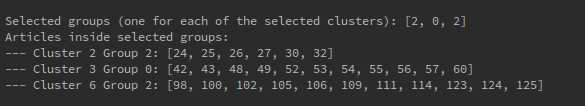
\includegraphics[scale=0.7]{static/figures/peloma/select3.png}}
    \caption{Επιλεγμένες ομάδες από κάθε κατηγορία.}
    \label{fig:select1}
\end{figure} 

Στην Εικόνα \ref{fig:select1} αποτυπώνονται οι ομάδες άρθρων που επιλέχθηκαν και οι οποίες μας οδήγησαν 
στην 1η φάση συστάσεων άρθρων. Μερικά από τα άρθρα εντός των επιλεγμένων ομάδων έχουν ήδη 
αναγνωσθεί από το χρήστη και είναι αυτά που οδήγησαν το σύστημα να συμπεράνει την ομοιότητα. 
Έτσι, γίνεται εύκολα αντιληπτό ότι εξαιτίας του περιορισμένου αριθμού άρθρων στη βάση δεδομένων, 
είναι πιθανό η ομοιότητα ενός χρήστη με μία κατηγορία να αυξάνεται καθώς αυτός συνεχίζει να 
επιλέγει άρθρα από την εν λόγω κατηγορία, όμως να μην υπάρχει διαθέσιμος ο επιθυμητός αριθμός 
άρθρων προς σύσταση. \\

Στον Πίνακα 5.2 αποτυπώνονται το ιστορικό ανάγνωσης του χρήστη, 
η τιμή ομοιότητας του χρήστη με κάθε κατηγορία άρθρων και η δεύτερη φάση συστάσεων. 
Παρατηρούμε πως ο χρήστης επέλεξε να αναγνώσει τόσο άρθρα από τις προτεινόμενες κατηγορίες, 
όσο και ένα άρθρο από την Κατηγορία {\en {\#5}}, εξ ου και η αύξηση της ομοιότητάς του με την κατηγορία αυτή. 
Το σύστημα εξακολουθεί να συμπεριφέρεται ορθά, δίνοντας μεγαλύτερη βαρύτητα στην Κατηγορία {\en {\#6}}. \\

% ============================ 2 ===================================

\begin{table}[h]
\centering
\begin{center}
\begin{tabular}{|c|c|c|c|}
\hline
\cellcolor{blizzardblue}{\textit{\en {2nd Recommendation}}}
& \multicolumn{1}{|p{3cm}|}{\centering \textbf{{\en {\# of articles }} \\ {\en {in user's}} \\ {\en {history}}}} 
& \multicolumn{1}{|p{3cm}|}{\centering \textbf{{\en {Similarity }} \\ {\en {with}} \\ {\en {Category}}}} 
& \multicolumn{1}{|p{3cm}|}{\centering \textbf{{\en {\# of }} \\ {\en {recommended articles}}}}\\
\hline
\multicolumn{1}{|p{3.9cm}|}{\centering \textbf{{\en {Category \#}1}}} & 4 & 0.2846 & 0 \\
\hline
\multicolumn{1}{|p{3.9cm}|}{\centering \textbf{{\en {Category \#}2}}} & 9 & 0.3273 & 0 \\
\hline
\rowcolor{classicrose}
\multicolumn{1}{|p{3.9cm}|}{\centering \textbf{{\en {Category \#}3}}} & \textbf{7} & \textbf{0.3566} & \textbf{2} \\
\hline
\multicolumn{1}{|p{3.9cm}|}{\centering \textbf{{\en {Category \#}4}}} & 4 &  0.2513 & 0 \\
\hline
\rowcolor{classicrose}
\multicolumn{1}{|p{3.9cm}|}{\centering \textbf{{\en {Category \#}5}}} & \textbf{5} & \textbf{0.3677} & \textbf{3} \\
\hline
\rowcolor{classicrose}
\multicolumn{1}{|p{3.9cm}|}{\centering \textbf{{\en {Category \#}6}}} & \textbf{5} & \textbf{0.3919} & \textbf{4} \\
\hline
\multicolumn{1}{|p{3.9cm}|}{\centering \textbf{{\en {Category \#}7}}} & 2 & 0.2696 & 0 \\
\hline
\end{tabular}
\caption{Ιστορικό ανάγνωσης και 2η φάση συστάσεων}
\end{center}
\label{table05.02}
\end{table}
% ====================================================================

\begin{comment}
Επιπρόσθετα, αξίζει να αναφέρουμε πως παρόλο που ο χρήστης επέλεξε να διαβάσει τα τρία προτεινόμενα 
άρθρα της Κατηγορίας {\en {\#2}}, φτάνοντας συνολικά στα εννιά διαβασμένα άρθρα από την κατηγορία αυτή, 
η ομοιότητά του με την εν λόγω κατηγορία υπολογίσθηκε τελικά μικρότερη σε σχέση με πριν. 
Επιλέγουμε να χρησιμοποιήσουμε το συγκεκριμένο σενάριο χρήσης του συστήματος και όχι κάποιο πιο ιδανικό, 
καθώς στην περίπτωση αυτή αναδεικνύεται ένα πρόβλημα των πιθανοτικών μοντέλων θεμάτων, όπου για κάθε άρθρο 
επιλέγουμε έναν αντιπροσωπευτικό αριθμό λέξεων και όχι ολόκληρο το κείμενό του.
Με τον ίδιο τρόπο επιδρούσαν τα μοντέλα θεμάτων πάνω στα {\en {clusters}} και τα {\en {groups}}, 
εξάγοντας έναν σαφώς μεγαλύτερο αριθμό αντιπροσωπευτικών λέξεων, που πιθανόν ``αδικεί'' 
ως προς το τελικό λεξιλόγιο κάποια από τα άρθρα που περιέχονται στα εν λόγω {\en {clusters}} και {\en {groups}}. 
Έτσι, αν οι λέξεις που χαρακτηρίζουν τα προσφάτως διαβασμένα άρθρα της Κατηγορίας {\en {\#2}} 
δεν αποτελούν μεγάλο μέρος του λεξιλογίου της κατηγορίας, είναι λογικό η ομοιότητα με την κατηγορία 
να μην αυξηθεί αισθητά και να μην έχουμε εκ νέου σχετικές συστάσεις. \\
\end{comment}

Στον Πίνακα 5.3 αποτυπώνονται το ιστορικό ανάγνωσης του χρήστη, 
η τιμή ομοιότητας του χρήστη με κάθε κατηγορία άρθρων και η τρίτη φάση συστάσεων. 
Παρατηρούμε πως το σύστημα λειτουργεί ομαλά, επιστρέφοντας ξανά συστάσεις 
από την Κατηγορία {\en {\#2}}, απ' όπου ο χρήστης έχει διαβάσει και το μεγαλύτερο 
αριθμό άρθρων. \\

\newpage 

% =============================== 3 =================================

\begin{table}[h]
\centering
\begin{center}
\begin{tabular}{|c|c|c|c|}
\hline
\cellcolor{blizzardblue}{\textit{\en {3rd Recommendation}}}
& \multicolumn{1}{|p{3cm}|}{\centering \textbf{{\en {\# of articles }} \\ {\en {in user's}} \\ {\en {history}}}} 
& \multicolumn{1}{|p{3cm}|}{\centering \textbf{{\en {Similarity }} \\ {\en {with}} \\ {\en {Category}}}} 
& \multicolumn{1}{|p{3cm}|}{\centering \textbf{{\en {\# of }} \\ {\en {recommended articles}}}}\\
\hline
\multicolumn{1}{|p{3.8cm}|}{\centering \textbf{{\en {Category \#}1}}} & 4 & 0.2853 & 0 \\
\hline
\rowcolor{classicrose}
\multicolumn{1}{|p{3.8cm}|}{\centering \textbf{{\en {Category \#}2}}} & \textbf{12} & \textbf{0.3837} & \textbf{2} \\
\hline
\multicolumn{1}{|p{3.8cm}|}{\centering \textbf{{\en {Category \#}3}}} & 8 & 0.3578 & 0 \\
\hline
\multicolumn{1}{|p{3.8cm}|}{\centering \textbf{{\en {Category \#}4}}} & 4 &  0.2779 & 0 \\
\hline
\rowcolor{classicrose}
\multicolumn{1}{|p{3.8cm}|}{\centering \textbf{{\en {Category \#}5}}} & \textbf{6} & \textbf{0.4013} & \textbf{3} \\
\hline
\rowcolor{classicrose}
\multicolumn{1}{|p{3.8cm}|}{\centering \textbf{{\en {Category \#}6}}} & \textbf{7} & \textbf{0.4026} & \textbf{4} \\
\hline
\multicolumn{1}{|p{3.8cm}|}{\centering \textbf{{\en {Category \#}7}}} & 2 & 0.3012 & 0 \\
\hline
\end{tabular}
\caption{Ιστορικό ανάγνωσης και 3η φάση συστάσεων}
\end{center}
\label{table05.03}
\end{table}
% ====================================================================

Το σύστημα καλύπτει επαρκώς τις αναγνωστικές ανάγκες του χρήστη, 
καθώς κατά τις τρεις διαφορετικές φάσεις έγιναν συστάσεις από τέσσερις διαφορετικές κατηγορίες άρθρων, 
από τις οποίες είχε διαβαστεί ένας σημαντικός αριθμός άρθρων. \\

% =======================================================================
Τέλος, ως μέρος της πειραματικής ανάλυσης επιλέγουμε να παραθέσουμε και ένα σενάριο χρήσης του συστήματος 
όπου ένας χρήστης με κενό αναγνωστικό ιστορικό 
συνδέεται στο σύστημα και επιλέγει προς ανάγνωση άρθρα μόνο από μία κατηγορία, 
την Κατηγορία {\en {\#}}1. 
Πρώτη επιλογή προς ανάγνωση αποτελεί το άρθρο {\en {\#}}12. \\
Σκοπός μας είναι να διαπιστώσουμε αν το σύστημα θα λειτουργήσει ορθώς, 
προτείνοντας στο χρήστη άρθρα μόνο από τη συγκεκριμένη κατηγορία, καθώς και να 
παρατηρήσουμε τον τρόπο με τον οποίο επιλέγονται τα άρθρα από το πιο όμοιο γκρουπ 
έως το λιγότερο όμοιο, καθώς ο χρήστης συνεχίζει την ανάγνωση  των προτεινόμενων άρθρων 
μέχρι την εξάντληση όλων των διαθέσιμων άρθρων της κατηγορίας αυτής. \\

\begin{figure}[!ht] \centering
\centerline{
    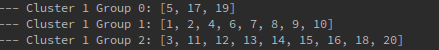
\includegraphics[scale=0.85]{static/figures/category/1.png}}
    \caption{{\en {Groups}} άρθρων της Κατηγορίας {\en {\#}}1.}
    \label{}
\end{figure} 

\begin{figure}[!ht] \centering
\centerline{
    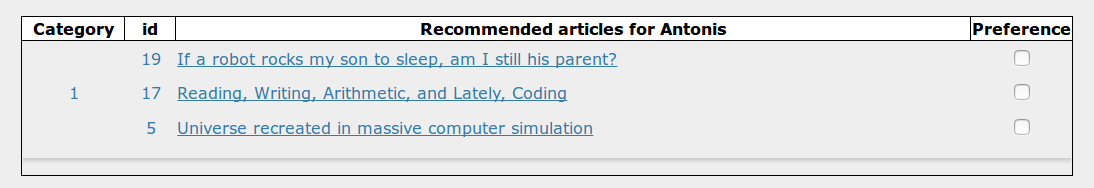
\includegraphics[scale=0.43]{static/figures/category/1a.png}}
    \caption{Κατηγορία {\en {\#}}1 - 1η σύσταση - Άρθρα από {\en {group 0}} .}
    \label{}
\end{figure} 

\begin{figure}[!ht] \centering
\centerline{
    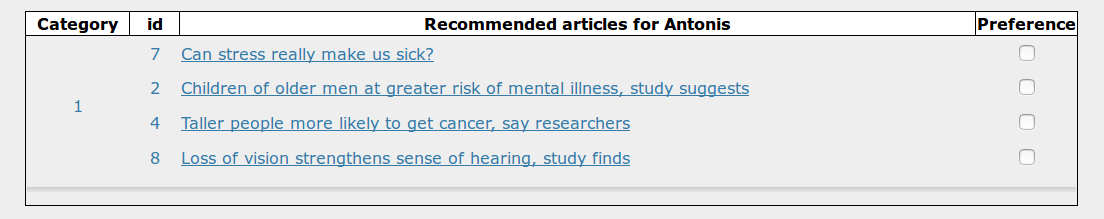
\includegraphics[scale=0.43]{static/figures/category/1b.png}}
    \caption{Κατηγορία {\en {\#}}1 - 2η σύσταση - Άρθρα από {\en {group 1}} .}
    \label{}
\end{figure} 

\begin{figure}[!ht] \centering
\centerline{
    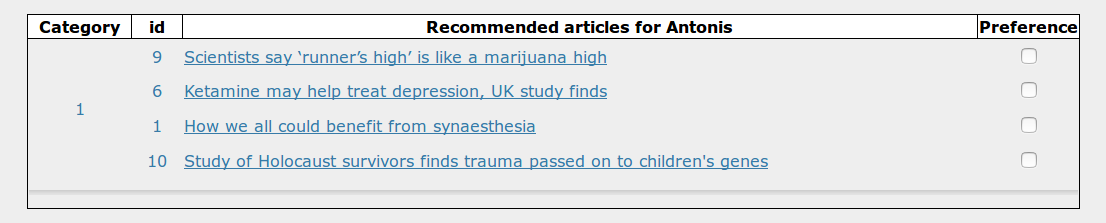
\includegraphics[scale=0.43]{static/figures/category/1c.png}}
    \caption{Κατηγορία {\en {\#}}1 - 3η σύσταση - Άρθρα από {\en {group 1}} .}
    \label{}
\end{figure} 
\begin{figure}[!ht] \centering
\centerline{
    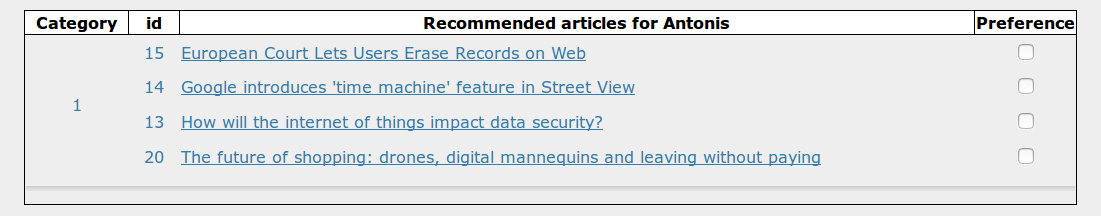
\includegraphics[scale=0.43]{static/figures/category/1d.png}}
    \caption{Κατηγορία {\en {\#}}1 - 4η σύσταση - Άρθρα από {\en {group 2}} .}
    \label{}
\end{figure} 

\begin{figure}[!ht] \centering
\centerline{
    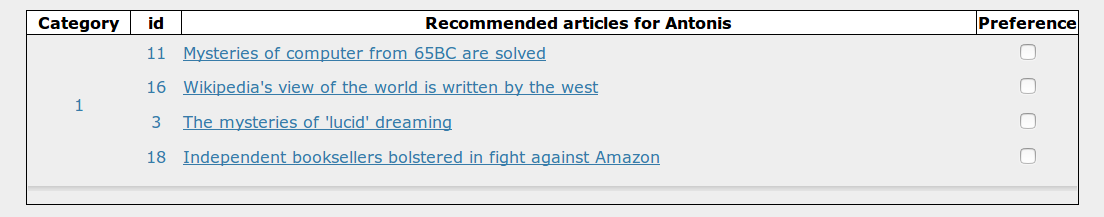
\includegraphics[scale=0.43]{static/figures/category/1e.png}}
    \caption{Κατηγορία {\en {\#}}1 - 5η σύσταση - Άρθρα από {\en {group 2}} .}
    \label{}
\end{figure} 

\newpage 

Κλείνοντας, η πειραματική αξιολόγηση έδειξε πως το σύστημα είναι σε θέση 
να καλύψει επαρκώς τις αναγνωστικές ανάγκες του χρήστη με βάση τα δεδομένα 
που του έχουν δοθεί ως είσοδος. 
Επιπλέον, μπορούμε να παρατηρήσουμε ότι σε ένα τέτοιο σύστημα 
είναι δύσκολο να πραγματοποιηθεί μια αντικειμενική αξιολόγηση, 
καθώς οι προτιμήσεις του χρήστη διαφέρουν από αυτές των υπολοίπων χρηστών 
ή ακόμα και από τις δικές του, ανάλογα με τις περιστάσεις. 
